% xjupiter-c3-2d-digraph.tex

\documentclass{standalone}
% jupiter-illustration-preamble.tex

\usepackage{tikz}
\usetikzlibrary{shapes, positioning, arrows.meta, calc, backgrounds, fit}

\def\hdist{1.8}
\def\vdist{2.0}
\tikzset{node distance = \vdist and \hdist}

\tikzset{every lower node part/.style = {red}}
\newcommand{\statesplit}[4]{% #1: state upper label; #2: state lower label; #3: position; #4: name
  \node (#4) [circle split, draw, minimum size = 6mm, text width = 10mm, align = center, #3, font = \Large]
  {
    $#1$
    \nodepart{lower}
    $#2$
  };
}

\newcommand{\rectsplit}[2]{% #1: state upper label; #2: state lower label
  \node [draw, rectangle split, rectangle split parts = 2, 
    align = center, font = \Large]
  {
    #1
    \nodepart{two}
    \textcolor{red}{#2}
  };
}

\newcommand{\transition}[4][]{% #2: start state; #3: end state; #4: transition label; #1: transition label position (optional)
  \draw[>=Stealth, ->] (#2) to node (#2to#3) [rectangle, draw, above = 2pt, sloped, #1, font = \small] {$#4$} (#3);
}

\newcommand{\set}[1]{\{#1\}}
\newcommand{\ins}[2]{\textsc{Ins}(#1,#2)}
\newcommand{\del}[2]{\textsc{Del}(#2)}
% \newcommand{\del}[2]{\textsc{Del}(#1,#2)}


\begin{document}
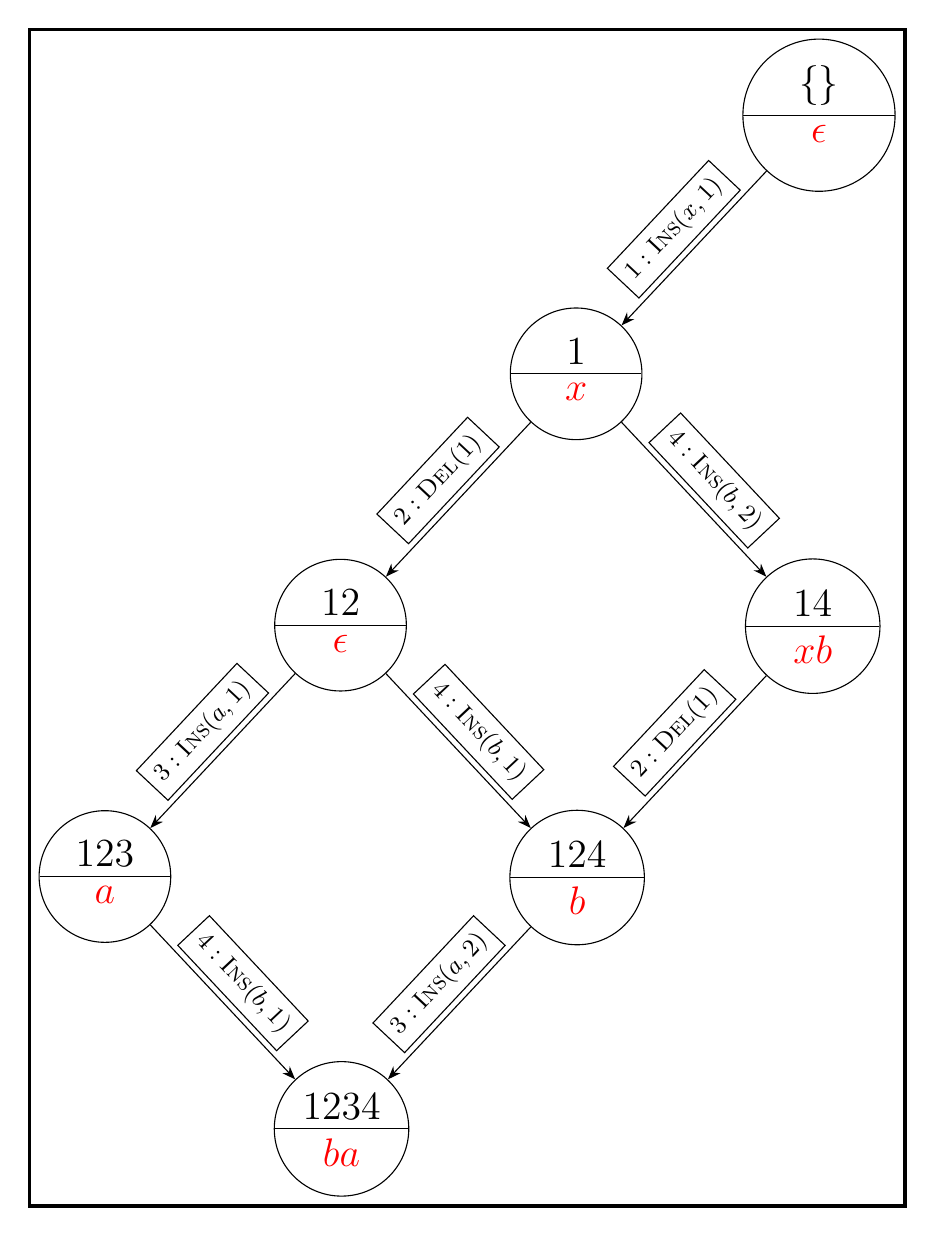
\begin{tikzpicture}[bg/.style = {rectangle, draw, very thick}]
  \statesplit{\{\}}{\epsilon}{}{0}
  \statesplit{1}{x}{below left = of 0}{1}
  \transition{0}{1}{1: \ins{x}{1}}
  \statesplit{12}{\epsilon}{below left = of 1}{12}
  \statesplit{14}{xb}{below right = of 1}{14}
  \statesplit{124}{b}{below right = of 12}{124}
  \statesplit{123}{a}{below left = of 12}{123}
  \statesplit{1234}{ba}{below right = of 123}{1234}
  \transition{1}{12}{2: \del{x}{1}}
  \transition{1}{14}{4: \ins{b}{2}}
  \transition{12}{124}{4: \ins{b}{1}}
  \transition{14}{124}{2: \del{x}{1}}
  \transition{12}{123}{3: \ins{a}{1}}
  \transition{124}{1234}{3: \ins{a}{2}}
  \transition{123}{1234}{4: \ins{b}{1}}

  \node () [fit = (0) (1) (12) (123) (14) (124) (1234), bg] {};

  % \node () [draw, red,  rotate fit = -45, fit = (1to14) (12to124) (123to1234),
  %   inner sep = 8pt,
  %   rectangle, rounded corners, loosely dashed, ultra thick] {};
\end{tikzpicture}
\end{document}